    In total there are 210 different CT images and 210 label masks. Each image consists of approximately 216 slices with an average size of 512:512. For the experiment the traditional 75 to 25 train-test split was used, resulting in 158 CT images for training and 52 CT images for validation. The training data consists of 13127 slices containing a kidney for training, while the test images contain 2700 slices with a kidney. The values of the training and test data are not significantly different, which can be seen in Figure \ref{fig:data_desc}. Label masks are encoded with three different values:
    \begin{itemize}
        \item 0 for background
        \item 1 for kidney
        \item 2 for tumor
    \end{itemize}
 For the purpose of this thesis, tumors are ignored and treated as background with value zero. Both, CT images and label masks are provided in an NIfTI \cite{Brainder..2012,Knipe.2005} file format. 
    


 \begin{figure}
 \centering
 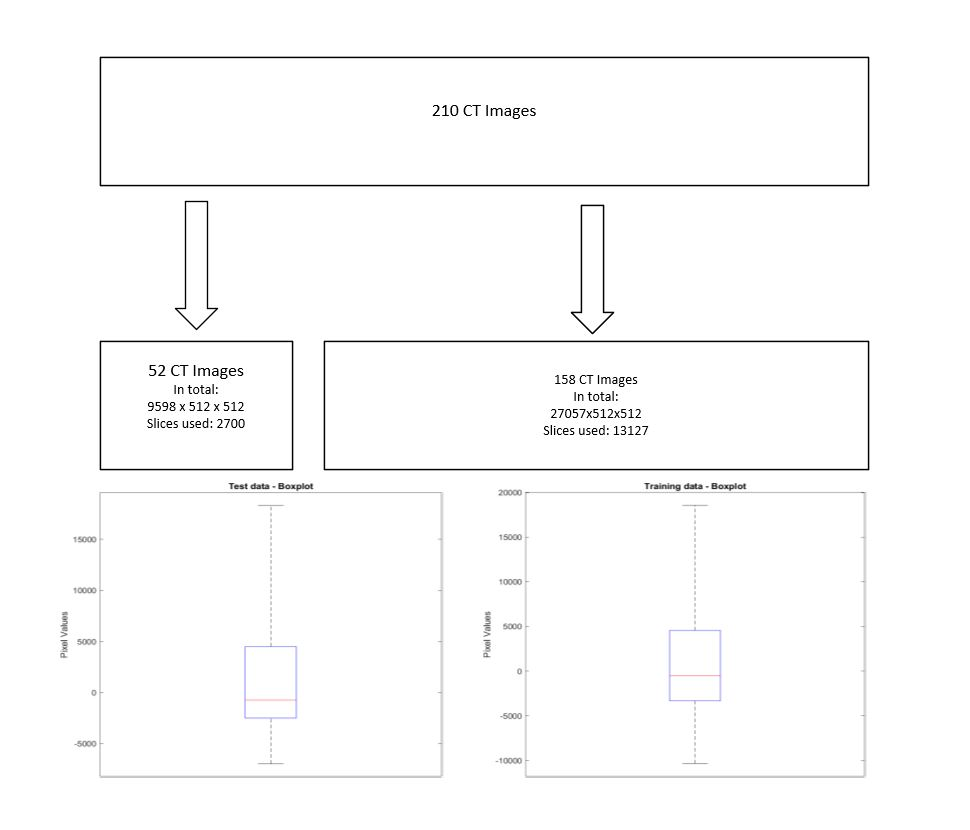
\includegraphics[width=0.7\linewidth]{PICs/data_desc.JPG}
 \caption{Data description - \textit{Test data:} Min: -6986, 1st: -1001, Median: -744, 3rd: -110, Max: 18326, Var: 348110; 
 \textit{Training data:} Min: -10240, 1st: -1003, Median: -540, 3rd: -109, Max: 18558, Var: 305240 }
 \label{fig:data_desc}
 \end{figure}

